% This is file `xampl-thesis.tex',
% generated with the docstrip utility.
%
% The original source files were:
%
% vakthesis.dtx  (with options: `xampl-thesis')
% 
% IMPORTANT NOTICE:
% 
% For the copyright see the source file.
% 
% Any modified versions of this file must be renamed
% with new filenames distinct from xampl-thesis.tex.
% 
% For distribution of the original source see the terms
% for copying and modification in the file vakthesis.dtx.
% 
% This generated file may be distributed as long as the
% original source files, as listed above, are part of the
% same distribution. (The sources need not necessarily be
% in the same archive or directory.)
% Існують кілька опцій, які необхідно вказувати як факультативний
% аргумент команди \documentclass. Наприклад, для докторської
% дисертації необхідно написати
% \documentclass[d]{vakthesis}

% Налагодження кодування шрифта, кодування вхідного файла
% та вибір необхідних мов
\documentclass[14pt]{vakthesis}
\usepackage{extsizes}
\usepackage{cmap} % для кодировки шрифтов в pdf
\usepackage[T1,T2A]{fontenc}
\usepackage[utf8]{inputenc}
% \usepackage{luaotfload}
%\usepackage[EU2]{fontenc}
%\usepackage{lmodern}

\usepackage[english,ukrainian,russian]{babel}

%usepackage{libertine}
% \usepackage[letterspace=-36]{microtype}

% Підключення необхідних пакетів. Наприклад,
% Пакети AMS для підтримки математики, теорем, спеціальних шрифтів

\usepackage{packages}
\allowdisplaybreaks


% Налагодження параметрів сторінки (зокрема берегів).
% Наприклад, за допомогою пакета geometry
\usepackage{geometry}
\geometry{hmargin={30mm,15mm},lines=29,vcentering}

% Якщо потрібно працювати лише з деякими розділами
%\includeonly{xampl-ch1,xampl-bib}

% Інформація про використані пакети тощо.
% Може знадобитися для відлагодження класу документа
%\listfiles
\makeatletter
\let\@Asbuk\@Alph
\let\@asbuk\@alph
\makeatother


% Титульна сторінка
\makeatletter
\def\onesupervisorname{Науковий\
    керівник}%
  \def\manysupervisorsname{Наукові\
    керівники}
\makeatother 

%\makeatletter
%\def\@maketitle{%
%  {\scshape
%   \@ifundefined{@institution@office}{\relax}{\@institution@office\par}
%   \@institution\par}
%  \vspace{\stretch{3}}%
%  {\raggedleft \@ifundefined{@secret}{}{\@secret\hfill}%
%     На правах\
%     рукопису \par}%
%  \vspace{\stretch{2}}%
%  {\bfseries\expandafter\emphsurname\@author \par}%
%  \vspace{\stretch{2}}%
%  {\raggedleft \CYRU\CYRD\CYRK\ \@udc \par}%
%  \vspace{\stretch{1}}%
%  {\large\bfseries\scshape \@title \par}%
%  \vspace{\stretch{2}}%
%  \@specialitycode\ --- \@specialityname\par
%  \vspace{\stretch{2}}%
%  Дисертація\
%    на\ здобуття\
%    вченої\
%    ступені\linebreak[1]%
%    \degreename\cyra\
%    \@science\par%?\linebreak[1]%
%  \vspace{\stretch{2}}%
%  {\raggedleft
%   \let\\\@format@person
%   \ifx\@supervisors\@empty
%     \hbox{}\hbox{}\hbox{}
%   \else
%     \@supervisors@caption\@supervisors\relax
%   \fi
%   \par}%
%  \vspace{\stretch{3}}%
%  \@town\ --- \@year}
%\def\@supervisors@caption{%
%  \ifnum\value{@supervisors@count}>1
%    \manysupervisorsname:%
%  \else
%    \onesupervisorname
%  \fi}
%\def\@format@person#1#2{\linebreak[4]%
%  \textbf{#1}, \linebreak[1]\@@format@person#2,,\@nil
%  \futurelet\next\@delimit@person}
%\def\@@format@person#1,#2,#3\@nil{#1%
%  \if\relax#2\relax\else, \linebreak[0]#2\fi}
%\def\@delimit@person{\ifx\relax\next\else,\fi}
%\def\emphsurname#1 #2{\textsc{#1} #2}
%\makeatother 

% Локальні означення
%\hyphenpenalty=10000

% NAMES
%% Переопределение именований %%%
\renewcommand{\abstractname}{Анотація}
% \renewcommand{\alsoname}{см. также}
\renewcommand{\appendixname}{Додаток}
\renewcommand{\bibname}{СПИСОК ВИКОРИСТАНИХ ИСТОЧНИКОВ}
% \renewcommand{\ccname}{исх.}
%\renewcommand{\chaptername}{Раздел}
\renewcommand{\chaptername}{РАЗДЕЛ}
\renewcommand{\contentsname}{СОДЕРЖАНИЕ}
% \renewcommand{\enclname}{вкл.}
\renewcommand{\figurename}{Рис.}
% \renewcommand{\headtoname}{вх.}
\renewcommand{\indexname}{Предметный указатель}
\renewcommand{\listfigurename}{Список рисунков}
\renewcommand{\listtablename}{Список таблиц}
%\renewcommand{\pagename}{Стр.}
\renewcommand{\partname}{Часть}
%\renewcommand{\refname}{СПИСОК ИСПОЛЬЗОВАННЫХ ИСТОЧНИКОВ}
% \renewcommand{\seename}{див.}
\renewcommand{\tablename}{Табл.}
% \renewcommand{\proofname}{Доказательство}
% \renewcommand{\algorithmcfname}{Алгоритм}% Update algorithm name
%
%% Настройка разделителей в содержании
%\renewcommand{\cftpartleader}{\cftdotfill{\cftdotsep}} % for parts
%\renewcommand{\cftchapleader}{~~\cftdotfill{\cftdotsep}} % for chapters
%\renewcommand{\cftsecleader}{\cftdotfill{\cftdotsep}} % for sections, if you really want! (It is default in report and book class (So you may not need it).


% COMMANDS
%
\newcommand{\bs}[1]{\ensuremath{\boldsymbol{#1}}}
\newcommand{\len}[1]{|#1|}
\newcommand{\pto}{\dashrightarrow}
\newcommand{\diver}{\!\uparrow}
\newcommand{\conver}{\!\downarrow}
\newcommand{\conveq}{\mathrel{\downarrow\!=}}
\newcommand{\var}[1]{\mbox{\texttt{#1}}}
%
\newcommand{\down}{\conver}
\newcommand{\downeq}{\conveq}
\newcommand{\pmaps}{\pto}
\newcommand{\conv}{\conver}


%=======================================
%

% Environments
% \theoremstyle{plain}
\newtheorem{problem}{Задача}[chapter]
\newtheorem{example}{Пример}[chapter]
\newtheorem{proposition}{Предложение}[chapter]
\newtheorem{corollary}{Следствие}[chapter]
\newtheorem{lemma}{Лемма}[chapter]
\newtheorem{theorem}{Теорема}[chapter]

% \theoremstyle{definition}
\newtheorem{definition}{Определение}[chapter]

% \theoremstyle{remark}
\newtheorem{remark}{Замечание}[chapter]
%================================================
% 
 

\begin{document}


% \setdefaultleftmargin{0pt}{}{}{}{}{}

% Назва дисертації
\title{Математичні імітаційні моделі для забезпечення узгодженості для розподілених сховищ даних}
% Прізвище, ім'я, по батькові здобувача
\author{Жолткевич Галина Григоріївна}
% Прізвище, ім'я, по батькові наукового керівника/консультанта
\supervisor{Рукас Кирило Маркович}
% Науковий ступінь, вчене звання наукового керівника/консультанта
           {доктор технічних наук, доцент}
% Спеціальність
%\speciality{01.05.02}
% Варіант із вказуванням факультативних аргументів
\speciality[Математичне моделювання та обчислювальні методи]{01.05.02}[технічних наук]
% Індекс за УДК
\udc{004.042/519.713.2}
% Установа, де виконана робота, і місто
\institution{Міністерство освіти і науки України \linebreak Харківський національний університет імені~В.Н.~Каразіна}{Харків}
% Рік, коли написана дисертація
\date{2019}

% Тут буде титульна сторінка
\maketitle

% Зміст
\tableofcontents

\chapter*{Вступ}

\paragraph{\bfseries Актуальність теми.}

В наше сьогодення інноваційні технології з'являються дуже швидко, а існуючі розвиваються з неймовірною швидкістю. Гіперлуп, багаточисленні дослідження космосу, наукові роботи в інших галузях, таких, 
як медицина, зелені мережі, а також, більш побутові, але все ще такі потрібні технології, такі, як 
комунікації, транспорт, розумні будинки... Не можна нехтувати тим фактом, що всі ці системи потребують
більшої гнучкості, швидкості, надійності та засобів для зберігання інформації також надійно та швидко і доступно, а інколи навіть доступність має бути майже у будь-якій точці земної кулі.
Тому одним з найважливіших компонентів для багатьох таких систем є швидке і надійне розподілене сховище.
В 21 столітті термін "розподілене сховище" становиться вже звичним. Деякі сховища збільшують кількість вузлів, деякі - ні. Причиною цьому є те, що багато з таких систем потребують сильної узгодженості даних. Але якщо збільшувати кількість вузлів для сховища, консистентність падає дуже швидко. А для деяких систем це важлива частина для їх стабільної роботи.

Бо є дуже відома CAP-теорема, яка стверджує, що неможливо одночасно задовільнити всі три 
характеристики для сховища, узгодженість (consistency), доступність (availability), 
стійкість до розділення (partition tolerance).

Ми не збираємося оскаржувати цю теорему, але робимо спробу обійти цю проблему. Механізм для цього і буде темою для цієї роботи.

\paragraph{\bfseries Взаємозв'язок роботи з науковими програмами, планами, темами.}
Диссертаційна робота виконана згідно з планом \linebreak
наково-дослідницьких работ Харківського Національного Університету ім.В.Н.Каразіна в рамках теми "Математичне и комп'ютерне моделювання процесів в розподілених базах даних" 
(номер государственной регистрации 0112U002098).


\paragraph{\bfseries Мета і завдання дослідження.}
Метою роботи являється побудува імітаційних та математичних моделей для механізму
підтримки сильної узгодженості у розподілених сховищах даних, проведення експериментів, оцінювання складності імітаційних моделей, побудува метрик, за якими можна дослідити складність даних моделей, а також розробка
обчислювальних методів для сформованого механізму. Це дозволить оцінити, наскільки можна розширити будь-яку розподілену систему і сформує методи для коректної роботи за такими умовами.

Для досягнення цієї мети у роботі розв'язані наступні задачі:
\begin{enumerate}[widest=9999,itemindent=*,leftmargin=0pt]
\item дослідження властивостей розподілених систем, зокрема, розподілених сховищ
\item дослідження критеріїв розподілених баз даних: узгодженості, доступності, стійкості
\item аналіз типів узгодженості
\item аналіз алгоритмів розповсюдження реплік
\item побудова математичної моделі для розподіленого сховщиа даних
\item доказ гіпотези про швидкість розповсюдження реплік
\item модель балансування узгоджених реплік
 
(пояснити які задачі були виконані шоб привести до актуальності задачі в цілому)

\end{enumerate}

\chapter{Теоретичні основи розподілених баз даних та цілісності даних}

Наскільки нам відомо, відповідно до CAP-теореми можна задовільнити тільки будь-які дві з трьох характеристик
для розподіленого сховища данихю
В цьому розділі розглядається можливість досягнути компромісу та забезпечити консистентні відповіді 
від бази даних, не втрачая доступності і стійкості для будь-якого сховища даних.
У цій частині ми пояснюємо гіпотезу, а далі проводимо дослідження, наскільки вдастся досягнути узгодженості завдяки
представлением маніпуляціям.

То ж давайте підійдемо ближче до суті.

Нехай у нас є розподілене сховище даних, що має N вузлів. Зараз ми не враховуємо функцію кожного вузла (мастер чи слейв) і 
вважаємо що кожний вузол приймає запити на читання і запис. Дозвольте нам сконцентруватися на механізмі обробки запитів.

Наша гіпотеза полягає в тому, що у сховищі даних узгодженість після запита на запис досягне достатнього значення с такою швидкістю, що сховище не встигне втратити доступності даних, і є можливість одночасно підтримувати узгодженість, коли відповіді на запити будуть балансувати тільки між вузлами, узгодженими між собою у даний момент часу, з достатньою швидкістю, у відповідь на запит конкретного юніта даних.
Мета цієї роботи полягає у оцінюванні значення узгодженості і доступності даних як результат роботи такого механізму, та алгоритму реалізації.

У цій частині, для того, щоб оцінити ефективність такого алгоритму, значення узгодженості і доступності, розглянемо ближче концепт цього рішення.
\section{Розподілені бази даних та їх типи узгодженості}

Розподілена база даних — це сукупність логічно взаємопов'язаних баз даних, розподілених у комп'ютерній мережі. Логічний зв'язок баз даних в розподіленій базі даних забезпечує система управління розподіленою базою даних, яка дозволяє управляти розподіленою базою даних таким чином, щоб створювати у користувачів ілюзію цілісної бази даних. 

Для будь-якої розподіленої бази даних існують такі властивості, встановлених К.Дейтом (https://studfiles.net/preview/5725402/page:15/):
\begin{itemize}
 \item Локальна автономія. Вона означає, що управління даними в кожному вузлі виконується локально і незалежно від інших вузлів системи
 \item Незалежність вузлів. Вважається, що в ідеальній системі всі вузли рівноправні і незалежні, а бази даних є рівноправними постачальниками інформації в загальний інформаційний простір.
 - Прозорість розміщення даних. Користувач не мусить знати де розміщені дані. Під час роботи створюється враження, що дані знаходяться саме на його комп’ютері.
 - Прозора фрагментація. Ця властивість трактується, як можливість створення фізично розподілених даних, які логічно утворюють єдине ціле. Допускається горизонтальна та вертикальна фрагментація.
 - Прозорість тиражування. Забезпечує тиражування (перенос змін) об’єктів первинної бази даних в усі вузли її розміщення внутрішньосистемними засобами.
 - Обробка розподілених запитів. Означає виконання операцій, сформованих, в рамках звичайного запиту на мові SQL.
 - Обробка розподілених транзакцій. Забезпечує виконання операцій з одночасним забезпеченням цілісності і узгодженості даних, шляхом використання двофазового протоколу фіксації транзакцій.
 - Незалежність від обладнання. Для оснащення вузла можуть використовуватися комп’ютери різних марок і виробників.
 - Незалежність від операційних систем. Передбачає допустимість взаємодії різноманітних операційних систем у різних вузлах розміщення розподіленої бази даних.
 - Прозорість мережі. Забезпечує будь-які протоколи в локальній обчислювальній мережі, яка обслуговує розподілену базу даних.
 - Незалежність від типу баз даних. Допускає співіснування різних систем керування базами даних.
 - Неперервність операцій. Дані доступні завжди, а операції над ними проводяться неперервно.

\end{itemize} 
http://citforum.ru/database/kbd96/45.shtml
Також для розподіленої бази даних існують три найважливіші парадигми, за допомогою яких підтримується ефективна робота для користувача:
\begin{itemize}
\item[Цілісність] Це складна проблема в розподіленій системі даних. Її рішення - синхронна і узгоджена зміна даних у кількох локальних базах даних, які скаладають розподілене сховище, і воно досягається застосуванням протокола фіксації транзакцій. Але це може застосовуватися у випадку, якщо база даних однородна. Якщо розподілена БД неоднородна, для цього використовують механізми розподілених транзакцій. Проте, це можливо при підтримці ХА-інтерфейсу учасниками обробки розподіленої транзакції, які функціонують на вузлах системи,   Это, однако, возможно, если участники обработки распределенной транзакции - СУБД, функционирующие на узлах системы. ХА-інтерфейс визначений в специфікації DTP консорціума X/Open. Нині XA-інтерфейс підтримується CA-OpenIngres, Informix, Microsoft SQL Server, Oracle, Sybase.
Якщо в розподіленому сховищі передбачено тиражування даних, це одразу пред'являє жорсткі  вимоги до підтримки цілісності на вузлах, куди направляються потоки тиражованих даних. То ж конфлікти щодо змін, які необхідно відслідковувати, неминучі. 
\item[Узгодженість] Як і у всіх інших розподілених систем, одним з основних компонентів цілісності даних (цілісності системи) є узгодженість - гарантія того, що усі вузли бачать однакові дані на будь-який момент часу.
Підтримка узгодженості в базах даних є ключовою при стабільній роботі розподіленого сховища даних. 
За узгодженістю слідують доступність даних (в будь-який момент кліент може отримати дані зі сховища або відповідь про те, що їх нема, за розумний обсяг часу) і стійкість до розділення системи (не зважаючи на розділення на ізольовані секції або втрати зв'язку з частиною вузлів, система не втрачає стабільність і здатність коректно відповідати на запити).

\end{itemize}



{\bfseries{red} Реплікація з книжки Таненбаума}
Є відома теорема CAP, яка наголошує, що з трьох властивостей (узгодженість (consistency), доступність (availability), стійкість до розділення (partition tolerance)) неможливо забезпечити більше двох в одній і тий самій конфігурації системи: наприклад, якщо забезпечити узгодженість, втратиться одна з двох інших властивостей. 

Крім того, в цій роботі важливо зазначити, що розділяють наступні моделі узгодженості:

\begin{itemize}
\item Сувора узгодженість (несуперечливість) (Strong Consistency) - на будь-який запит на читання елемента даних $x$ сховище дає значення, які відповідає наойновішої версії. Це найжорсткіша, але модель несуперечливості для підтримки абсолютної узгодженості, і її забезпечення до втрачання вкличини доступності для даної конфігурації сховища даних.

\item Послідовна несуперечливість (sequential consistency) - результат будь-якої дії такий же, якщо б операції читання та запису всіх процесів у сховище даних виконувались би в деякому послідовному порядку і притому операції кожного окремого процесу виконувались би у порядку, визначеного його програмою. Тобто будь-яке правильне чередування операцій читання и запису є допустимим , але всі процеси бачать одне и те ж чередування операцій.

\item Причинна несуперечливість (causal consistency) - операції на запис, які потенціально зв'язані причинно-наслідковим зв'язком, повинні  обслуговуватися всіма процесами в одному і тому ж порядку, а паралельні записи можуть параллельно обслуговуватися на разних вузлах в різному порядку.

\item Несуперечливість FIFO. Операції запису, які здійснюються поодиноким процесом, розглядаються іншими процесами в тому порядку, в якому вони здійснюються, але операції запису з різних процесів, можуть спостерігатися різними процесами у різному порядку.

\item Потенціальна несуперечливість - при відсутності змін всі репліки поступово стають несуперечливими. Такі моделі використовуються, коли клієнт запрошує завжди одну й ту ж репліку та записи в таке сховище виконуються нечасто.


\end{itemize}

Забезпечення суворої узгодженості - занадто дорога модель для будь-якої розподіленої бази даних, хоча деякі бази це забезпечують, для яких застосування такої моделі - сувора технічна вимога, що випливає з бізнес-логіки продукту, де така база використовується.
Але такі конфігурації розподілених БД втрачають значення іншої характеристики - доступності даних, бо для великих БД потрібно багато часу, щоб досягнути суворої несуперечливості і клієнт змушений чекати, щоб мати гарантію на отримання несуперечливих актуальних даних.

Ми намагаємося знайти компроміс, щоб максимально близько реалізувати таку модель без втрачання доступності і стійкості до розділення розподіленої бази (див. модель реалізації  у наступних частинах).

\section{Використання різних моделей несуперечливості у реалізаціях розподілених баз даних}
\section{Балансування навантаження}

Балансувальник навантаження - це метод, який дозволяє розподіляти задачі між мережевими пристроями з метою оптимізації використання ресурсів, збереження часу відопвіді на запити, горизонтального масштабування кластеру та забезпечення відмовостійкості розподіленої системи. Прикладами пристроїв, до яких може бути застосований цей метод, є серверні кластери, проксі-сервери, межмережеві екрани, комутатори, сервери інспектування вмісту, сервери DNS, мережеві адаптери. Балансувальник запиту може бути застосований у різних цілях, також деякі реалізації балансування - проекти з відкритими джерелами, які дозволяють дописати необхідний функціонал для перенаправлення запитів за необхідним алгоритмом, допрацювати існуючі алгоритми та інше (HAProxy, Nginx, Seesaw, Zevent, Neutrino, Traefik, тощо https://geekflare.com/open-source-load-balancer/).
\begin{figure}
\centering
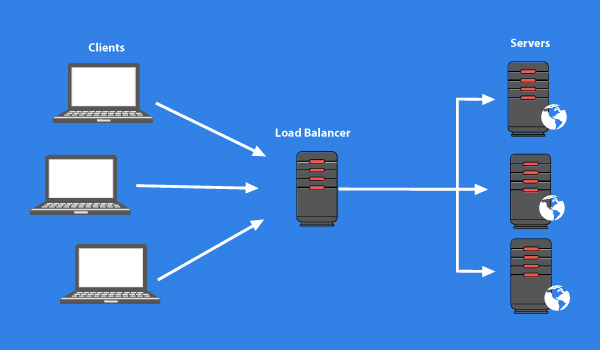
\includegraphics[width=\linewidth]{images/load-balancing-general.jpg}
     \caption{Загальна архітектура балансування навантаження.}
     \label{fig:lb_general}
\end{figure}

Малюнок \ref{fig:lb_general} демонструє загальний механізм роботи  балансувальника навантаження: запит приходить спочатку на проміжний вузел (або кластер) і далі  перенаправляється на один з вузлів в системі, який спроможний відповісти на запит клієнта. Періодично балансувальник робе так званий "healthcheck", щоб вчасно мати знання про те, які вузли зможуть відповісти на запит.
Балансування може здійснятися за різними додатковими характеристиками: запит відправиться на найбільш незайнятий вузел, на вузел, який за показниками процесора на даний момент часу має не завантажений процесор, тощо.

Алгоритми балансування навантаження загалом можна класифікувати наступним чином (Малюнок \ref{fig:lb_classification}):

\begin{figure}
\centering
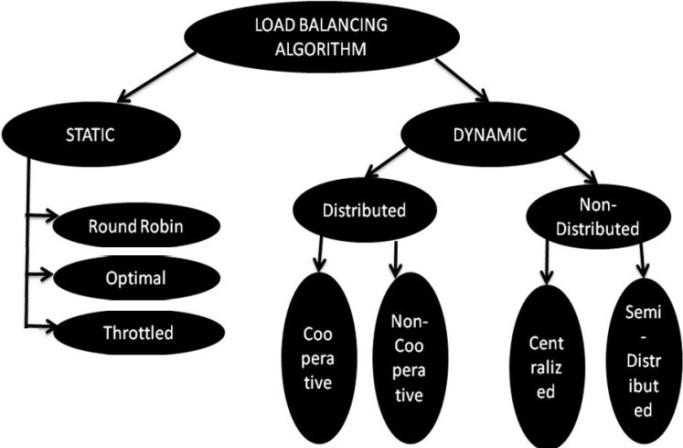
\includegraphics[width=\linewidth]{images/Classification-of-load-balancing-algorithms-in-cloud.png}
     \caption{Класифікація алгоритмів балансування навантаження.}
     \label{fig:lb_classification}
\end{figure}

Ці алгоритми спершу розділяють на статичні і динамічні
\begin{enumerate}
\item Статичне балансування. В цьому підході балансування навантаження реалізується через забезпечення важливої інформації про систему. Визначається продуктивність вузла на початку виконання операцій. Вузли виконують обчислювання та надають результати на інші вузли. Потім навантаження, яка 


Static Load Balancing: In this approach load balancing is achieved by providing priori information about the system. The
performance of the node is determined at the commencement of execution. Nodes calculate their allotted work and submit the
result to remote node. Then depending on the performance work load is distributed in start without considering the current load
[13]. Static load balancing methods are non-preemptive i.e. once the load is allocated to the node it cannot be transferred to
another node. This method requires less communication hence reduces the execution time [16]. The main drawback of this
approach is that it does not take current state of the system while making allocation decisions. This has the major impact on the
overall performance of the system due to load fluctuation in distributed system [18].There are three types of static load
balancing algorithms: round robin, central manager, threshold algorithm and randomized algorithm

\end{enumerate}

\chapter{Маршрутизація запитів у розподіленій системі даних. Порівняльна характеристика}
Розподілена база даних (РБД) ‒ це множина логічно взаємозалежних баз даних, розподілених у комп’ютерній мережі.
(Більше про це написати  )
% https://elearning.sumdu.edu.ua/free_content/lectured:89b3d175c06a6b137e410cb14821d0e94549ad5a/latest/44605/index.html).

Розподілені бази даних  скаладаються з N розподілених машин, які об'єднують у різні групи - кластери або ж просто в окремі незалежні вузли комп'ютерної мережі.
Так чи інакше є методи, які дозволять керувати запитами і їх пунктами призначення:
 - балансування навантаження - програма, яка дозволяє розподілити клієнтські запити між вузлами системи з метою оптимального (найшвидшого, найдешевшого, тощо) оброблення запиту
 - альтернативою є власні програми, які працюють на кожному вузлі і виконують функції перенаправлення запиту на інший релевантний вузол
 - гібрідний механізм, який поєднує в собі рішення балансування навантаження і власних програм з тим функціоналом, якого не вистачає тому чи іншому балансувальнику навантаження.

У цій роботі ми також намагаємося знайти краще рішення для перенаправлення запитів за необхідним нам алгоритмом і оцінимо всі варіанти реалізації. Для цього нам потрібно детальніше розібратися, за якими схемами можуть діяти балансувальники навантаження.


% Потім Описати що також само можна відправляти запит на узгоджений вузел

\section{Балансувальник навантаження як рішення керування запитами у розподіленому сховищі}

Балансувальник навантаження - це метод, який дозволяє розподіляти задачі між мережевими пристроями з метою оптимізації використання ресурсів, збереження часу відопвіді на запити, горизонтального масштабування кластеру та забезпечення відмовостійкості розподіленої системи. Прикладами пристроїв, до яких може бути застосований цей метод, є серверні кластери, проксі-сервери, межмережеві екрани, комутатори, сервери інспектування вмісту, сервери DNS, мережеві адаптери. Балансувальник запиту може бути застосований у різних цілях, також деякі реалізації балансування - проекти з відкритими джерелами, які дозволяють дописати необхідний функціонал для перенаправлення запитів за необхідним алгоритмом (HAProxy, Nginx, Seesaw, Zevent, Neutrino, Traefik, etc. https://geekflare.com/open-source-load-balancer/).


Малюнок 1 демонструє загальний механізм роботи  балансувальника навантаження: запит приходить спочатку на проміжний вузел (або кластер) і далі  перенаправляється на один з вузлів в системі, який спроможний відповісти на запит клієнта. Періодично балансувальник робе так званий "healthcheck", щоб вчасно мати знання про те, які вузли зможуть відповісти на запит.
Балансування може здійснятися за різними додатковими характеристиками: запит відправиться на найбільш незайнятий вузел, на вузел, який за показниками процесора на даний момент часу має не завантажений процесор, тощо.

Є наступні техніки балансування між вузлами у розподіленій системі:

описати техніки round robin, least response , ...

описати техніку оновлення таблиці з вузлами, які пройшли healthcheck

пояснити проблему, чому наразы не підтримується те, що потрібно нам : таблиця вузлів динамічна і змінюється постійно, описати проблеми, які можуть виникнути, чому не можна повністю розраховувати на балансувальник (або опенсорс)

\section{Концептуальні моделі Власний алгоритм та його оцінка}
порівняти з рішенням балансувальника
\section{Концептуальні моделі Гібрідний}
порівняти з рішенням балансувальника і власного алгоритму


моделі трьох рішень

\section{Математичні моделі балансування узгодженості}
\section{Імітаційні моделі балансування узгодженості}
реалізація
\section{Оцінка несуперечливості, доступності за застосованими моделями}
\section{Інші існуючі методи реалізації}

\chapter{Дослідження часу збіжності несуперечливості у ідеальному сховищі}

\chapter{Висновки}
\section{Потенціал використання моделей балансування узгодженості в розподілених сховищах даних}
Підвищення значення узгодженості при збереженні значення доступності розподіленої системи

\end{document}
